\documentclass[a4paper,11pt]{article}
\usepackage[polish]{babel}
\usepackage[OT4]{fontenc}
\usepackage[utf8]{inputenc}
\usepackage[pdftex]{graphicx}
\usepackage{epstopdf}

\begin{document}
Jakub Bartodziej, 291470
\section{Podejście do problemu}
\subsection{Gdybyśmy znali wszystkie parametry}

Manager bufetu chce zmaksymalizować zysk, więc dobrze byłoby tak dobierać ceny,
żeby wartość oczekiwana zysku z każdego była największa. Można zastanawiać się nad wariancją, 
albo odchyleniem standardowym - jest ryzyko, że rzeczywiste wartości będą się
znacząco odchylać od średniej - zostawmy ten problem na chwilę.

Niech $Z_{\beta}$ będzie zmienną losową oznaczającą, zysk z jednego dnia przy
cenie $\beta$. Zachodzi:
\[
EZ_{\beta} = (10 - \beta)\sum_{i=1}^{N}([\alpha_i \le \beta]p^+_i + [\alpha_i > \beta]p^-_i)
\]
Gdzie $(\alpha_i, p^-_i ,p^+_i)$ to trójka opisująca klienta. Ponieważ klienci są w grupach
to wyrażenie
\[
\sum_{i=1}^{N}([\alpha_i \le \beta]p^+_i + [\alpha_i > \beta]p^-_i)
\]
będące wartością oczekiwaną liczby klientów którzy zdecydowali się na zakup traktowane jako funkcja $\beta$ zmienia wartości jedynie w kilku punktach - $\cup_i\{\alpha_i\}$. Na przedziałach stanowiących resztę zbioru są zatem plateau. A największa wartość $EZ_{\beta}$
jest osiągana z lewej strony takiego przedziału z powodu czynnika $(10 - \beta)$.

Wykres wartości funkcji przyporzątkowującej cenie oczekiwaną liczbę kupujących dla
zestawu grup: \\

\begin{table}[ht] 
\centering

\begin{tabular}{c|c|c}
$\alpha$ & $p^-$ & $p^+$\\
\hline
$2.471852$ & $0.04148218$ & $0.8432869$ \\
$5.290343$ & $0.37199400$ & $0.6152462$ \\ 
$5.284968$ & $0.37079776$ & $0.5885168$ \\
$6.630816$ & $0.28899424$ & $0.9853943$
\end{tabular}

\end{table}

\includegraphics[scale=.4, angle=270]{plateau.eps}

Uzasadniony (trochę chaotycznie) jest więc wzór:
\[
max_{\beta \in [0; 10]}EZ_{\beta} = max_{\beta \in \{0, \alpha_1, ..., \alpha_{\#grup}\}}EZ_{\beta}
\]
Jeśli znamy wszystkie parametry to, żeby zmaksymalizować zysk wystarczy więc zawsze ustalać cenę $\beta$, dla której $EZ_{\beta}$ jest największa. Ponadto lepszej wartości oczekiwanej
nie da się uzyskać.

Wróćmy do problemu odchyleń od średniej - ponieważ zawsze sumujemy tu sporo podobnych składników - co najmniej 48 takich samych zmiennych losowych zerojedynkowych (nie było
to napisane explicite, ale $p_-$ i $p_+$ to wartości oczekiwane takich właśnie
zmiennych) nie warto zajmować się przypadkiem szczególnie dużych odchyleń.
\subsection{Jak oceniać strategię}
Opisana powyżej strategia jest w pewnym sensie optymalna, jednak nasz menedżer nie może
jej zrealizować, bo nie zna wartości parametrów. Może się ona jednak przydać przy
ocenie strategii ją aproksymującej. Można spojrzeć, jak bardzo udało się zbliżyć
z wartością oczekiwaną łącznego zysku do maksymalnej wartości oczekiwanej łącznego zysku.
Dobrze byłoby też podawać wariancję łącznego zysku - nasz manager może nie być
skłonny do ryzyka.

Niestety analityczne obliczenie tych wartości może się okazać trudne, ale za pomocą
R można zasymulować działanie takiej strategii n razy i policzyć średnią i wariancję
wyniku, albo narysować jakiś wykres.

\section{Szczególne sytuacje}

\subsection{Bardzo małe M}
W takiej sytuacji trudno wymyślić cokolwiek mądrego, bo nie ma żadnych użytecznych
informacji na temat parametrów klientów bufetu, więc można stosować strategie trywialne,
jak np: stosowanie zawsze tylko jednego kosztu, albo losowanie kosztu z przedziału [0, 10]
z jakimś rozkładem prawdopodobieństwa.

\subsection{Bardzo duże M}
Tutaj manager ma pewien komfort, bo może estymować wartości parametrów klientów
przez stosunkowo długi czas i dni wykorzystane na eksperymentowanie nie odbiją się
bardzo negatywnie na średnim dziennym wyniku. W szczególności łatwe staje się zbadanie
podziału klientów na grupy: po pewnym czasie klienci z poszczególnych grup kupili obiady
podobną ilość razy. W obrębie grupy można zastosować jakiś estymator jej parametrów,
na przykład MLE. Ten pomysł przeniknął do jednej z proponowanych strategii.

\section{Proponowane strategie}
\subsection{Bisekcja}
Ta strategia przyjmuje dodatnią liczbę naturalną $k$ jako argument, wykonuje po $k$ prób w
obydwu połowach badanego przedziału kosztów i zawęża przedział do tej połowy, która
dała większy zysk i powtarza te kroki aż do wyczerpania liczby prób (dni).

Intuicja prowadząca do wymyślenia tej metody była następująca:
można zdefiniować wartości oczekiwane zysku dla kosztu losowanego z danego przedziału, a
$k$ losowych prób przybliża taką wartość oczekiwaną. Z dwóch przedziałów lepszy wydaje
się taki, który ma większą wartość oczekiwaną zysku.

Niestety może zdarzyć się tak, że istnieje mały przedział dający duży zysk wśród
dużych przedziałów dających mały zysk i ta metoda go nie wyłapie. Z powodu tego,
że jest mały trudno go jednak wychwycić. Alternatywnie taka metoda mogłaby zawężać
obszar wyszukiwania do przedziału, który ma większe maksimum dziennego zysku, co
pozwoliłoby zapobiec sytuacji, gdy bardzo małe dzienne zyski ,,ściągają'' średnią w dół.

\subsection{Plateau}
W sekcji 1.1 znalazła się wzmianka o tym, że wartość oczekiwana liczby klientów którzy zdecydowali się na zakup danego dnia traktowana jako funkcja kosztu posiłku posiada
plateau (jest ich $\#$grup$+ 1$). Z powodów tam opisanych, gdybyśmy umieli oceniać
gdzie znajdują się te plateau to możnaby było wybrać jako koszt taki początek jednego
z nich, który daje największą wartość oczekiwaną dziennego zysku.

Strategia Plateau $k$ razy losuje koszt z przedziału $[0, 10]$ z rozkładem jednostajnym
i wykonuje z tym kosztem eksperyment na klientach bufetu. Pod koniec $k$-tego dnia mamy 
$k$ par (koszt, $\#$kupionych obiadów). Iterujemy po punktach w kolejności rosnących
kosztów. Do jednego plateau zaliczamy punkty o większym koszcie różniące się liczbą
kupionych obiadów o nie więcej niż wartość parametru $d1$ i skaczemy na koniec nowoutworzonego plateau. Następnie wybiera się takie plateau, które maksymalizuje ilość
kupionych obiadów i do wyczerpania liczby dni ustala cenę $=$ początek tego plateau + $d2$.

\subsection{Zgadywanie podziału na grupy i MLE}
Podobnie, jak w strategii Plateau pomysł polega na eksperymentowaniu przy użyciu
kosztów losowanych z rozkładem jednostajnym z przedziału $[0, 10]$. Po $k$ próbach
uznajemy, że jesteśmy w stanie wyznaczyć podział na grupy - sortujemy klientów po
liczbie zakupów i uznajemy, że otrzymany ciąg jest dobrym przybliżeniem poszczególnych grup
ustawionych jedna za drugą.

Po podziale na grupy dla każdej z nich zostanie zastosowany MLE w celu wyznaczenia
jej parametrów. Tworzymy wektor par (cena, $\#$klientów w grupie, która kupiła obiad), 
ozn. $(\beta_i, g_i)$, $g$ to klientów w grupie.

Funkcja wiarygodności wygląda następująco:

\[
L((\alpha, p^-, p^+), (\beta_1, g_1), (\beta_2, g_2), ..., (\beta_g, g_g)) =
\]

\[
\prod_{i=1}^{g}[\beta_i \ge \alpha]((p^+)^{g_i}(1-p^+)^{g - g_i}) +
               [\beta_i < \alpha]((p^-)^{g_i}(1-p^-)^{g - g_i})
\]

Można zapisać to trochę prościej. Oznaczmy:

\begin{itemize}
\item przez $a$ liczbę przypadków, kiedy klient kupił obiad po cenie niższej, niż $\alpha$,
\item przez $b$ liczbę przypadków, kiedy klient kupił obiad po cenie wyższej, niż $\alpha$,
\item przez $c$ liczbę przypadków, kiedy klient nie kupił obiadu po cenie niższej, niż $\alpha$,
\item przez $d$ liczbę przypadków, kiedy klient nie kupił obiadu po cenie wyższej, niż $\alpha$. 
\end{itemize}

Wtedy:

\[
L(...) = (p^-)^{a}(p^+)^{b}(1 - p^-)^{c}(1 - p^+)^{d}
\]

\[
\log(L(...)) = a\log(p^-) + b\log(p^+) + c\log(1 - p^-) + d\log(1 - p^+)
\]

Ta funkcja ogólnie jest nieciągła, ale można szukać jej maksimum na przedziałach
$(0, \beta_1), (\beta_1, \beta_2), ..., (\beta_g, 10)$ i wziąć maksimum z tych
wartości.

Po wyestymowaniu parametrów dla każdej grupy można już skorzystać dla
nich ze strategii optymalnej z sekcji 1.1. Wyznaczonego kosztu można używać już
do końca.

\subsection{Kwantyle}
Kolejna strategia z eksperymentowaniem. Przyjmuje parametry $k$ i $q$. Wykonuje
$k$ losowych prób z kosztami losowanym z rozkładem jednostajnym z przedziału $[0, 10]$.
Następnie do końca losuje cenę spośród tych, dla których zysk znajdował się w $q*100\%$
największych.

\section{Implementacja}

\subsection{Strategie}
Strategie zostały zaimplementowane w osobnych plikach bisect.R, plateau.R, mle.R i quantiles.R.
Reszta narzędzi znajduje się w pliku statystyka.R. Do ,,tworzenia'' strategii
służą ,,konstruktory'': create.*.strategy(...), które przyjmują różne argumenty
będące parametrami strategii. Wygodnie jest trakować strategie o różnych parametrach
jako różne i osobno je testować. Ze względu na ograniczenia sprzętowe przetestowałem
dla niewielkiej ilości strategii.

\subsection{Badanie jakości strategii i prezentacja wyników}
Załączony wykres obrazują sytuację dla pewnego podzbioru strategii i możliwych liczb dni.
Został on wygenerowany przez kod zamieszczony w pliku plots.R. Dla każdego
rozmiaru grupy generuję parametry dla $10$ różnych zestawów grup klientów. Potem stosuję
każdą strategię na tych zestawach dla każdego $n \in \{5, 20, 50, 200\}$. $1000$ odpuściłem,
bo za długo by się liczyło. Na wykresie zamieszczam punkty będące ilorazem zysku i 
maksymalnej wartości oczekiwanej zysku. Znajduje się on w pliku plot.eps.

\section{Analiza strategii i interpretacja wykresów}
Wykresy bardzo wyraźnie prezentują zachowanie strategii w zależności od n i liczby grup.
Postaram się jakoś skomentować to co można tam zobaczyć.

W praktycznie każdej strategii wariancja zmniejsza się wraz ze wzrostem n. Jest to tym,
że duża liczba prób pozwala znacznie lepiej przybliżyć wartość oczekiwaną zysku podczas
stosowania danej strategii.

\subsection{Kwantyle, $k=5, q=0.85$}
Zdecydowanie najgorsza z testowanych strategii. Dla $k = 1, 2, 3$ jej zyski niemal równomiernie
rozrzucone są po przedziale $[0; 1]$ masksymalnej wartości oczekiwanej zysku (mwoz.).
Co ciekawe najlepiej zachowuje się dla $k = 4$. Interpretacja: wybieranie tej
z $5$ początkowych cen, które dały najlepsze wyniki po prostu jest zbyt słabym
przybliżeniem optymalnej ceny.

\subsection{Plateau, $k=10, d1=20, d2=0.5$}
Daje w miarę solidne wyniki w górnej części przedziału, znów lepiej jest dla dużych $k$.
Niestety, Są opatrzone dużą wariancją. Generalnie lepsze wyniki daje dla dużych n.
Interpretacja: $10$ strzałów to za mało, żeby wiarygodnie wyznaczyć plateau funkcji
wartości oczekiwanej ilości kupionych obiadów od ceny. Dużo prostsza ,,Bisekcja''
przynosi znacznie lepsze wyniki dla dużych $k$ i $n$.

\subsection{Bisekcja, $k = 4$}
Bisekcja mimo swojej prostoty całkiem nieźle radzi sobie dla dużych n. Co ciekawe lepsze
i bardziej skupione wyniki osiąga dla większej ilości grup. Moja interpretacja:
liczba grup powoduje, że trudniej ustalić cenę, która odpowiada wszystkim kilentom,
przez co zmniejsza się maksymalna wartość oczekiwana. Strategia dobierania ceny
na podstawie wyników wydaje się przynosić w takiej sytuacji lepsze i bardziej skupione efekty.
Dla małych n i dużych k bisekcja osiąga rezultaty prawie wyłącznie powyżej $0.5$ maksymalnej
wartości oczekiwanej, co można uznać za przyzwoity wynik.

\subsection{MLE, $k = 15$}
Bardzo dobre wyniki zarówno dla małych, jak i dużych $n$ i $k$, w miarę nieznaczna wariancja,
poza tym podobny do swojej wersji z mnieszym $k$.

\subsection{MLE, $k = 5$}
Niekwestionowany król wszystkich strategii. Nieprawdopodobne wydaje się, że dla $k$ równego 5
można wiarygodnie wyznaczyć podział na grupy i na jego podstawie dobrze wyestymować parametry
grup. Okazuje się również, że zmniejszenie $k$ pozwala osiągać lepsze wyniki! Praktycznie
dla każdego rozmiaru grupy i każej wartości n wyniki są świetne, a wariancja mała. Interpretacja:
zmniejszenie $k$ poprawia wyniki, bo strategia ma już wystarczającą ilość informacji do wybrania
dobrej ceny i może wcześniej zacząć czerpać z tego korzyści. MLE to jedyna strategia, która wykorzystuje
wszystkie informacje, jakie otrzymuje o klientach bufetu i jako jedyna korzysta z
zaawansowanego narzędzia statystycznego :). Na miejscu managera zainteresowałbym się
tą strategią.

\end{document}
